\documentclass{beamer}
\usepackage{graphicx}
\usepackage{amssymb,amsfonts,amsmath}
% \usepackage{tikz,tkz-euclide}
\usepackage{subcaption}
% \usepackage{parskip}
% \usetikzlibrary{arrows.meta}
% \usetikzlibrary{calc,patterns}
\usefonttheme[onlymath]{serif}
% \usetheme{Berlin}
\title{Weekly Report}
\author{WU Zihan}
\begin{document}
\maketitle
% \begin{frame}
%     \frametitle{Outline}
%     \tableofcontents
% \end{frame}

\section{Probability Model}
\begin{frame}
    \frametitle{Probability Model}
    % two columns
    \begin{columns}
        \begin{column}{0.5\textwidth}

            \begin{itemize}
                \item Target: Reconstruct biclusters in big matrix;
                \item Method: Partition the matrix into small blocks and reconstruct biclusters in each block larger than $T_m \times T_n$;
                \item Probability Model: We construct the probability model to decide $T_p$ re-partition times to ensure the probability of missing biclusters is less than $\epsilon$.
            \end{itemize}
        \end{column}
        \begin{column}{0.5\textwidth}
            \vspace{-1cm}
            \centering
            \begin{figure}[htb]
                \centering
                \begin{subfigure}[b]{\textwidth}
                    \centering
                    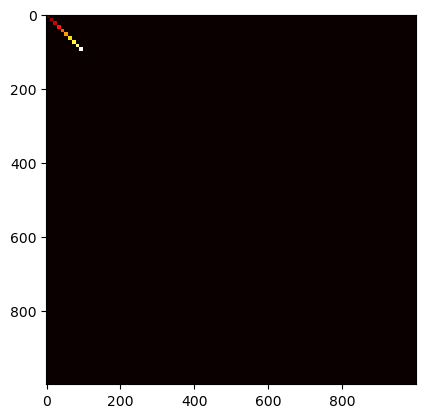
\includegraphics[width=0.6\linewidth]{A.png}
                    \caption{Original matrix $A$}
                    \label{fig:image1}
                \end{subfigure}
                % \vspace{-0.5cm}
                \begin{subfigure}[b]{\textwidth}
                    \centering
                    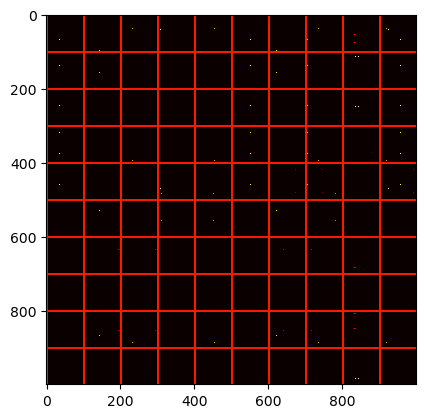
\includegraphics[width=0.6\linewidth]{partition.png}
                    \caption{Partition matrix $A$ into blocks}
                    \label{fig:image2}
                \end{subfigure}
                \vspace{-0.8cm}
                % \caption{Probability Model}
                % \label{fig:comparison}
            \end{figure}
        \end{column}
    \end{columns}
\end{frame}

\section{Results}
\begin{frame}
    \frametitle{Results for simulated data matrix}
    \begin{columns}[T]
        \begin{column}{0.5\textwidth}
            \centering
            \textbf{Experiment settings}
            \begin{itemize}
                \item $A \in \mathbb{R}^{M\times N}$, $M = N = 1000$
                \item Biclusters number $K = 10$
                \item Bicluster height $\phi_1 = \phi_2 = \cdots = \phi_K = \phi$
                \item Bicluster width $\psi_1 = \psi_2 = \cdots = \psi_K = \psi$
                \item Threshold $T_m = T_n = 4$
            \end{itemize}
        \end{column}
        \begin{column}{0.5\textwidth}
            \textbf{Experiment results}
            $$ T_p \ge \frac{\ln(1 - p_0)}{-2 [m\phi (s^{(k)})^2+ n\psi (t^{(k)})^2]} $$
            \begin{itemize}
                \item
                      According to computation, $T_p \ge 303.024$ to ensure the probability of missing biclusters is less than $1\%$.
                \item
                      We set $T_p = 304$ and do $1000$ experiments, in which $992$ successful detections are observed.
            \end{itemize}
        \end{column}
    \end{columns}
\end{frame}

%two columns, each one is a picture. picfile names are `Tp.pdf' and `numofsuc.pdf'
\begin{frame}
    \frametitle{Results}
    \begin{columns}[T]
        \begin{column}{0.5\textwidth}
            \centering
            \textbf{$T_p$ numbers for various bicluster sizes}
            \begin{figure}[htb]
                \centering
                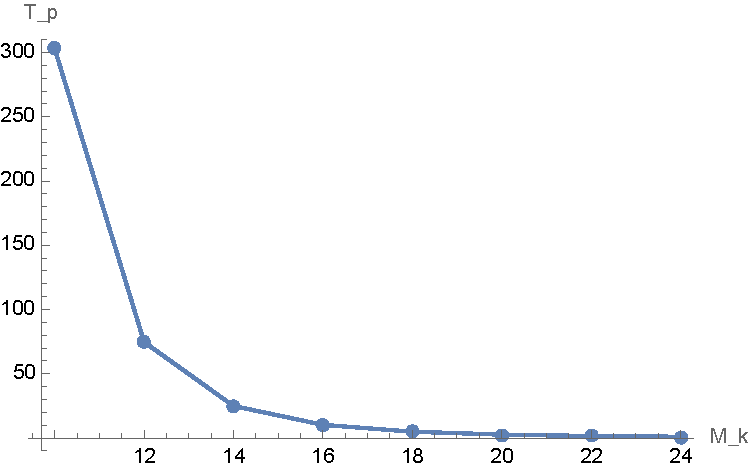
\includegraphics[width=0.8\linewidth]{Tp.pdf}
                \caption{$T_p$ numbers for various bicluster sizes}
                \label{fig:image3}
            \end{figure}
        \end{column}
        \begin{column}{0.5\textwidth}
            \textbf{Rate of successful detections}
            Each $M_k$ is tested $100$ times.
            \begin{figure}[htb]
                \centering
                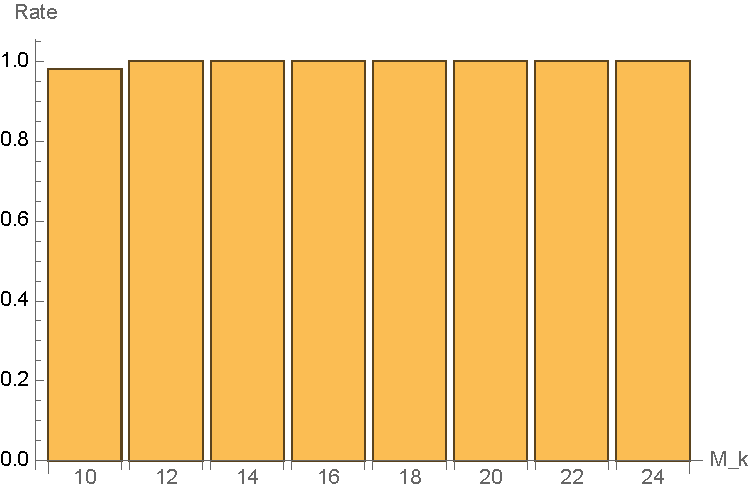
\includegraphics[width=0.8\linewidth]{numofsuc.pdf}
                \caption{Rate of successful detections}
                \label{fig:image4}
            \end{figure}
        \end{column}
    \end{columns}
\end{frame}

\end{document}